This project aims to extend \textbf{Cosys-AirSim}, an open-source framework built upon Microsoft's AirSim simulator, which provides high-fidelity, physics-based environments for autonomous vehicles. 
While the current framework offers robust tools for simulating either Unmanned Aerial Vehicles (UAVs) or Unmanned Ground Vehicles (UGVs), it is restricted to single-domain operations, forcing users to choose only one vehicle type per simulation instance.
The current inability of Cosys-AirSim to support concurrent UAV and UGV simulation creates a bottleneck for researchers and industries needing to validate multi-domain systems in a unified virtual space.
\begin{figure}[H]
\centering
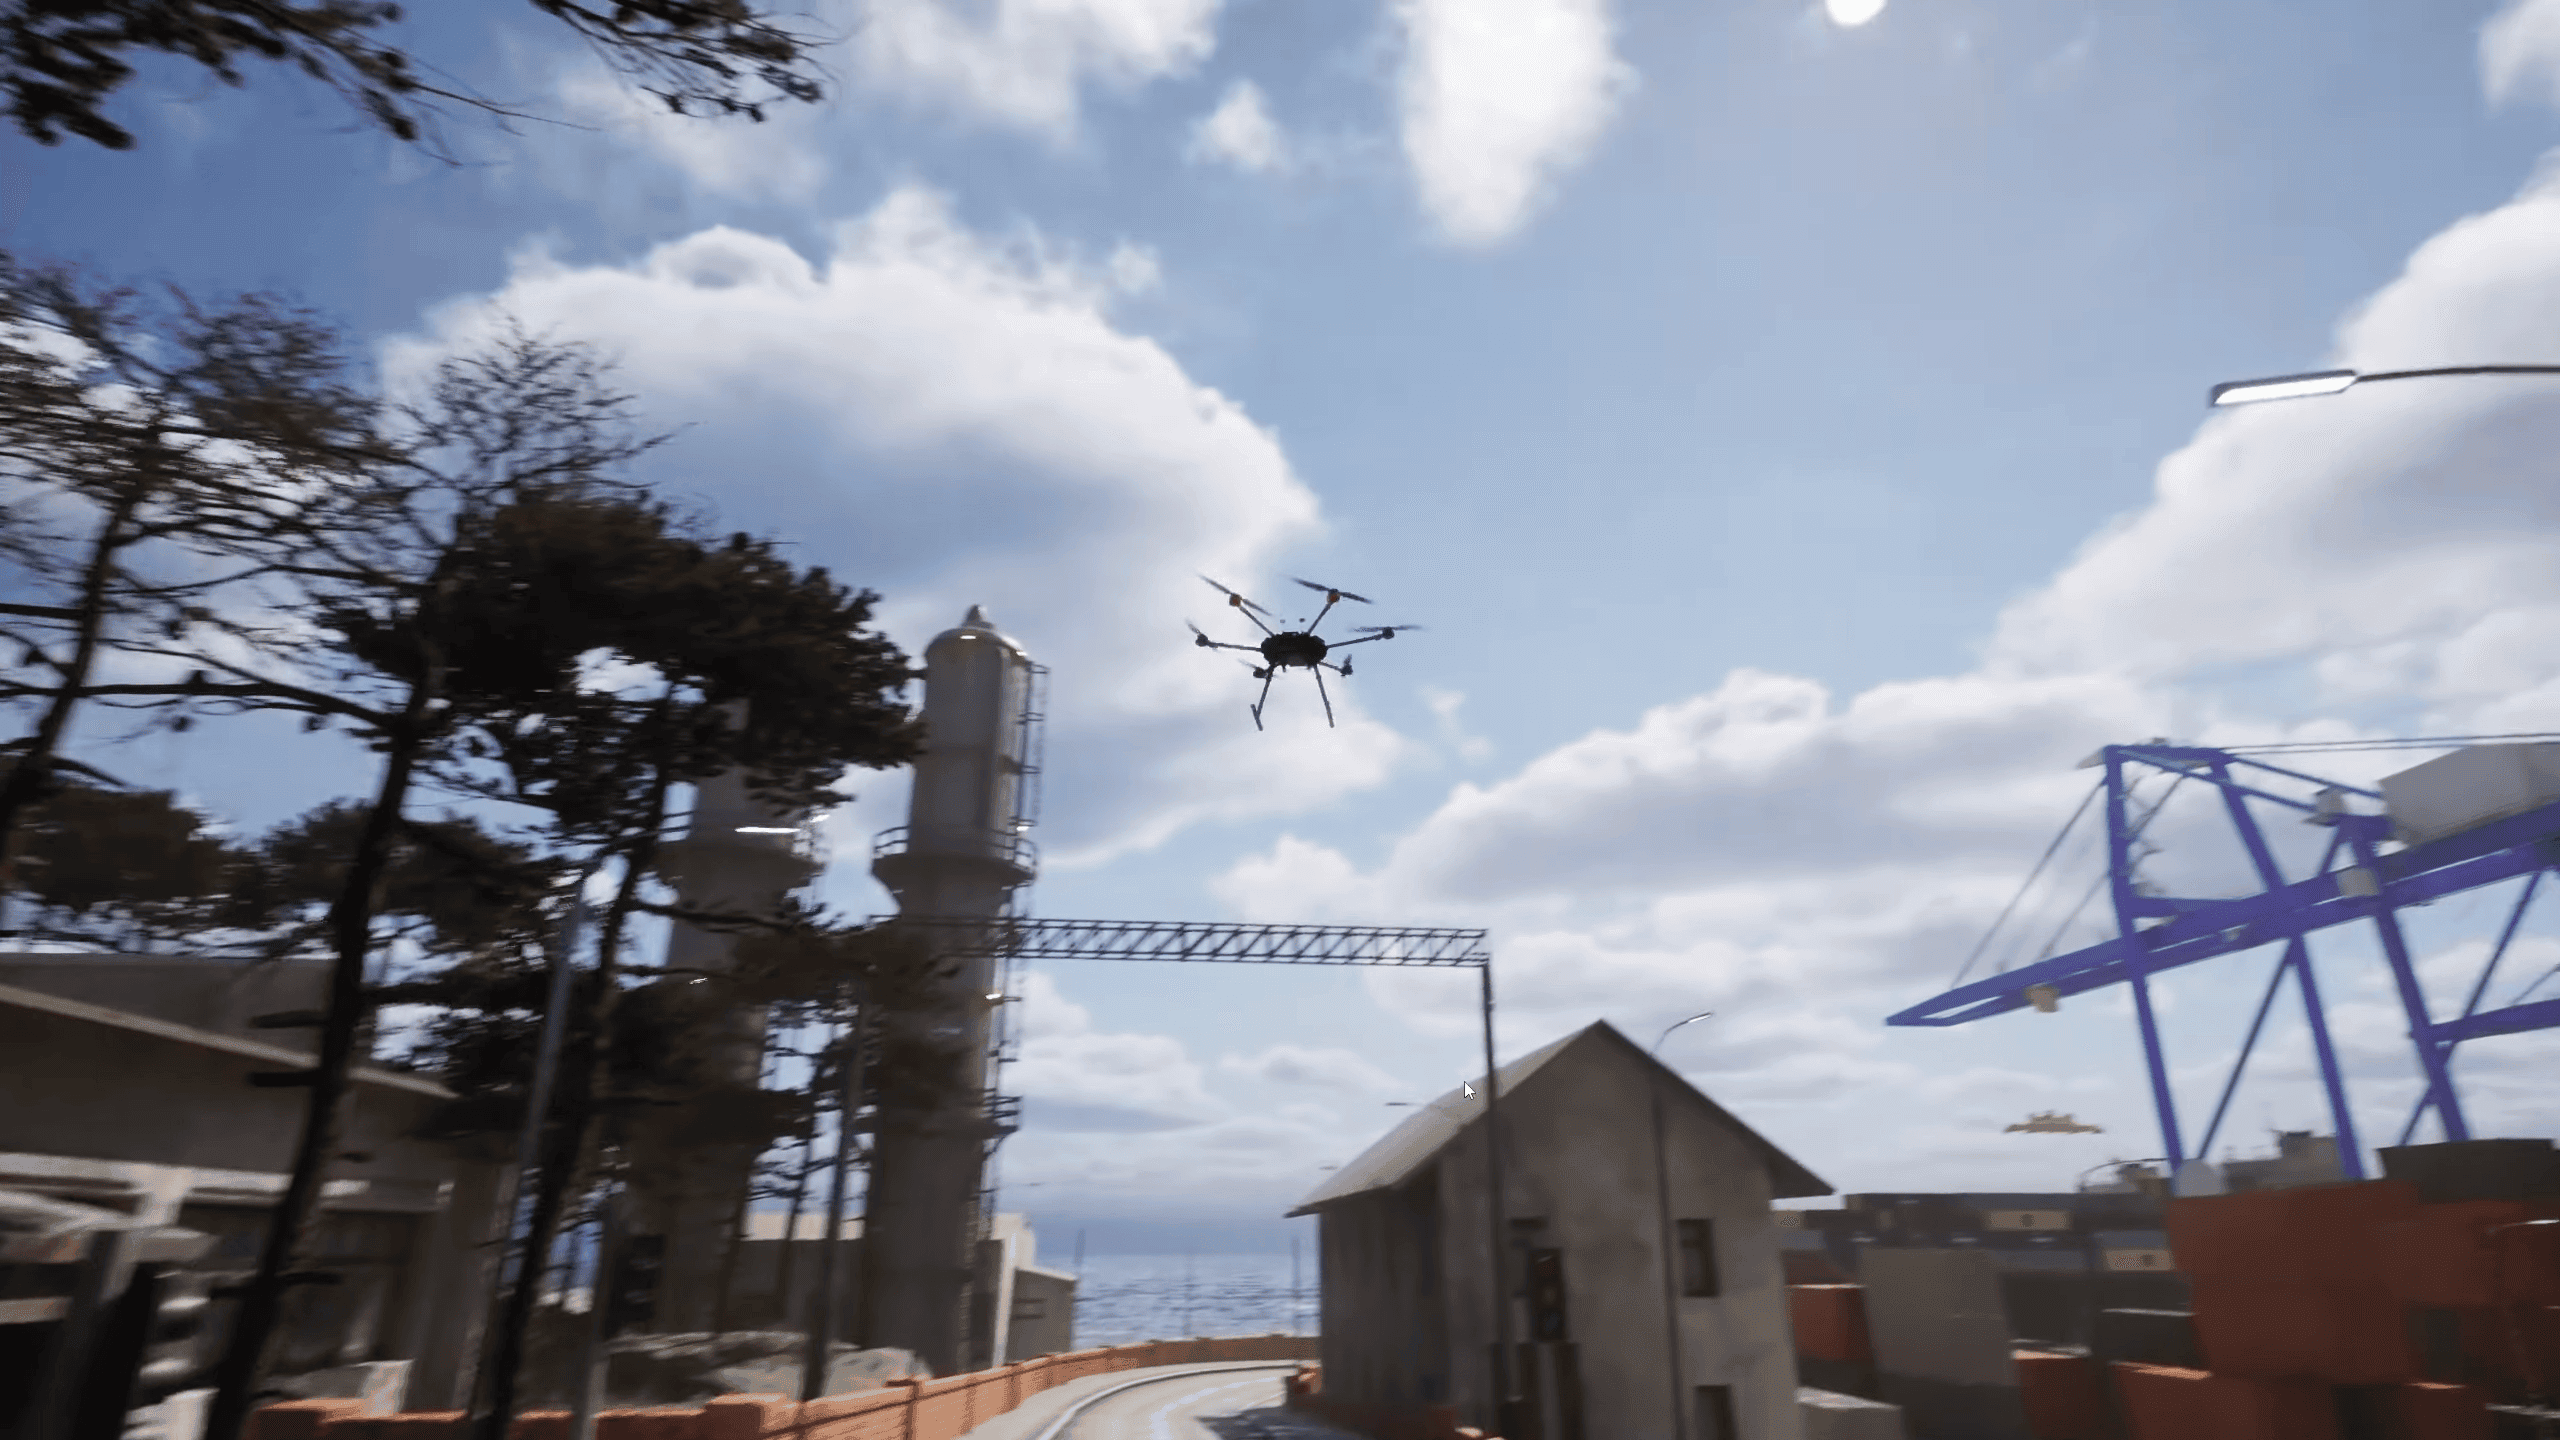
\includegraphics[width=0.4\textwidth]{graphics/Cosys_Airsim_UAV_example.png}
\caption{Example view of a UAV produced by Cosys-AirSim.}
\label{fig:UAV_example_view}
\end{figure}
\begin{figure}[H]
\centering
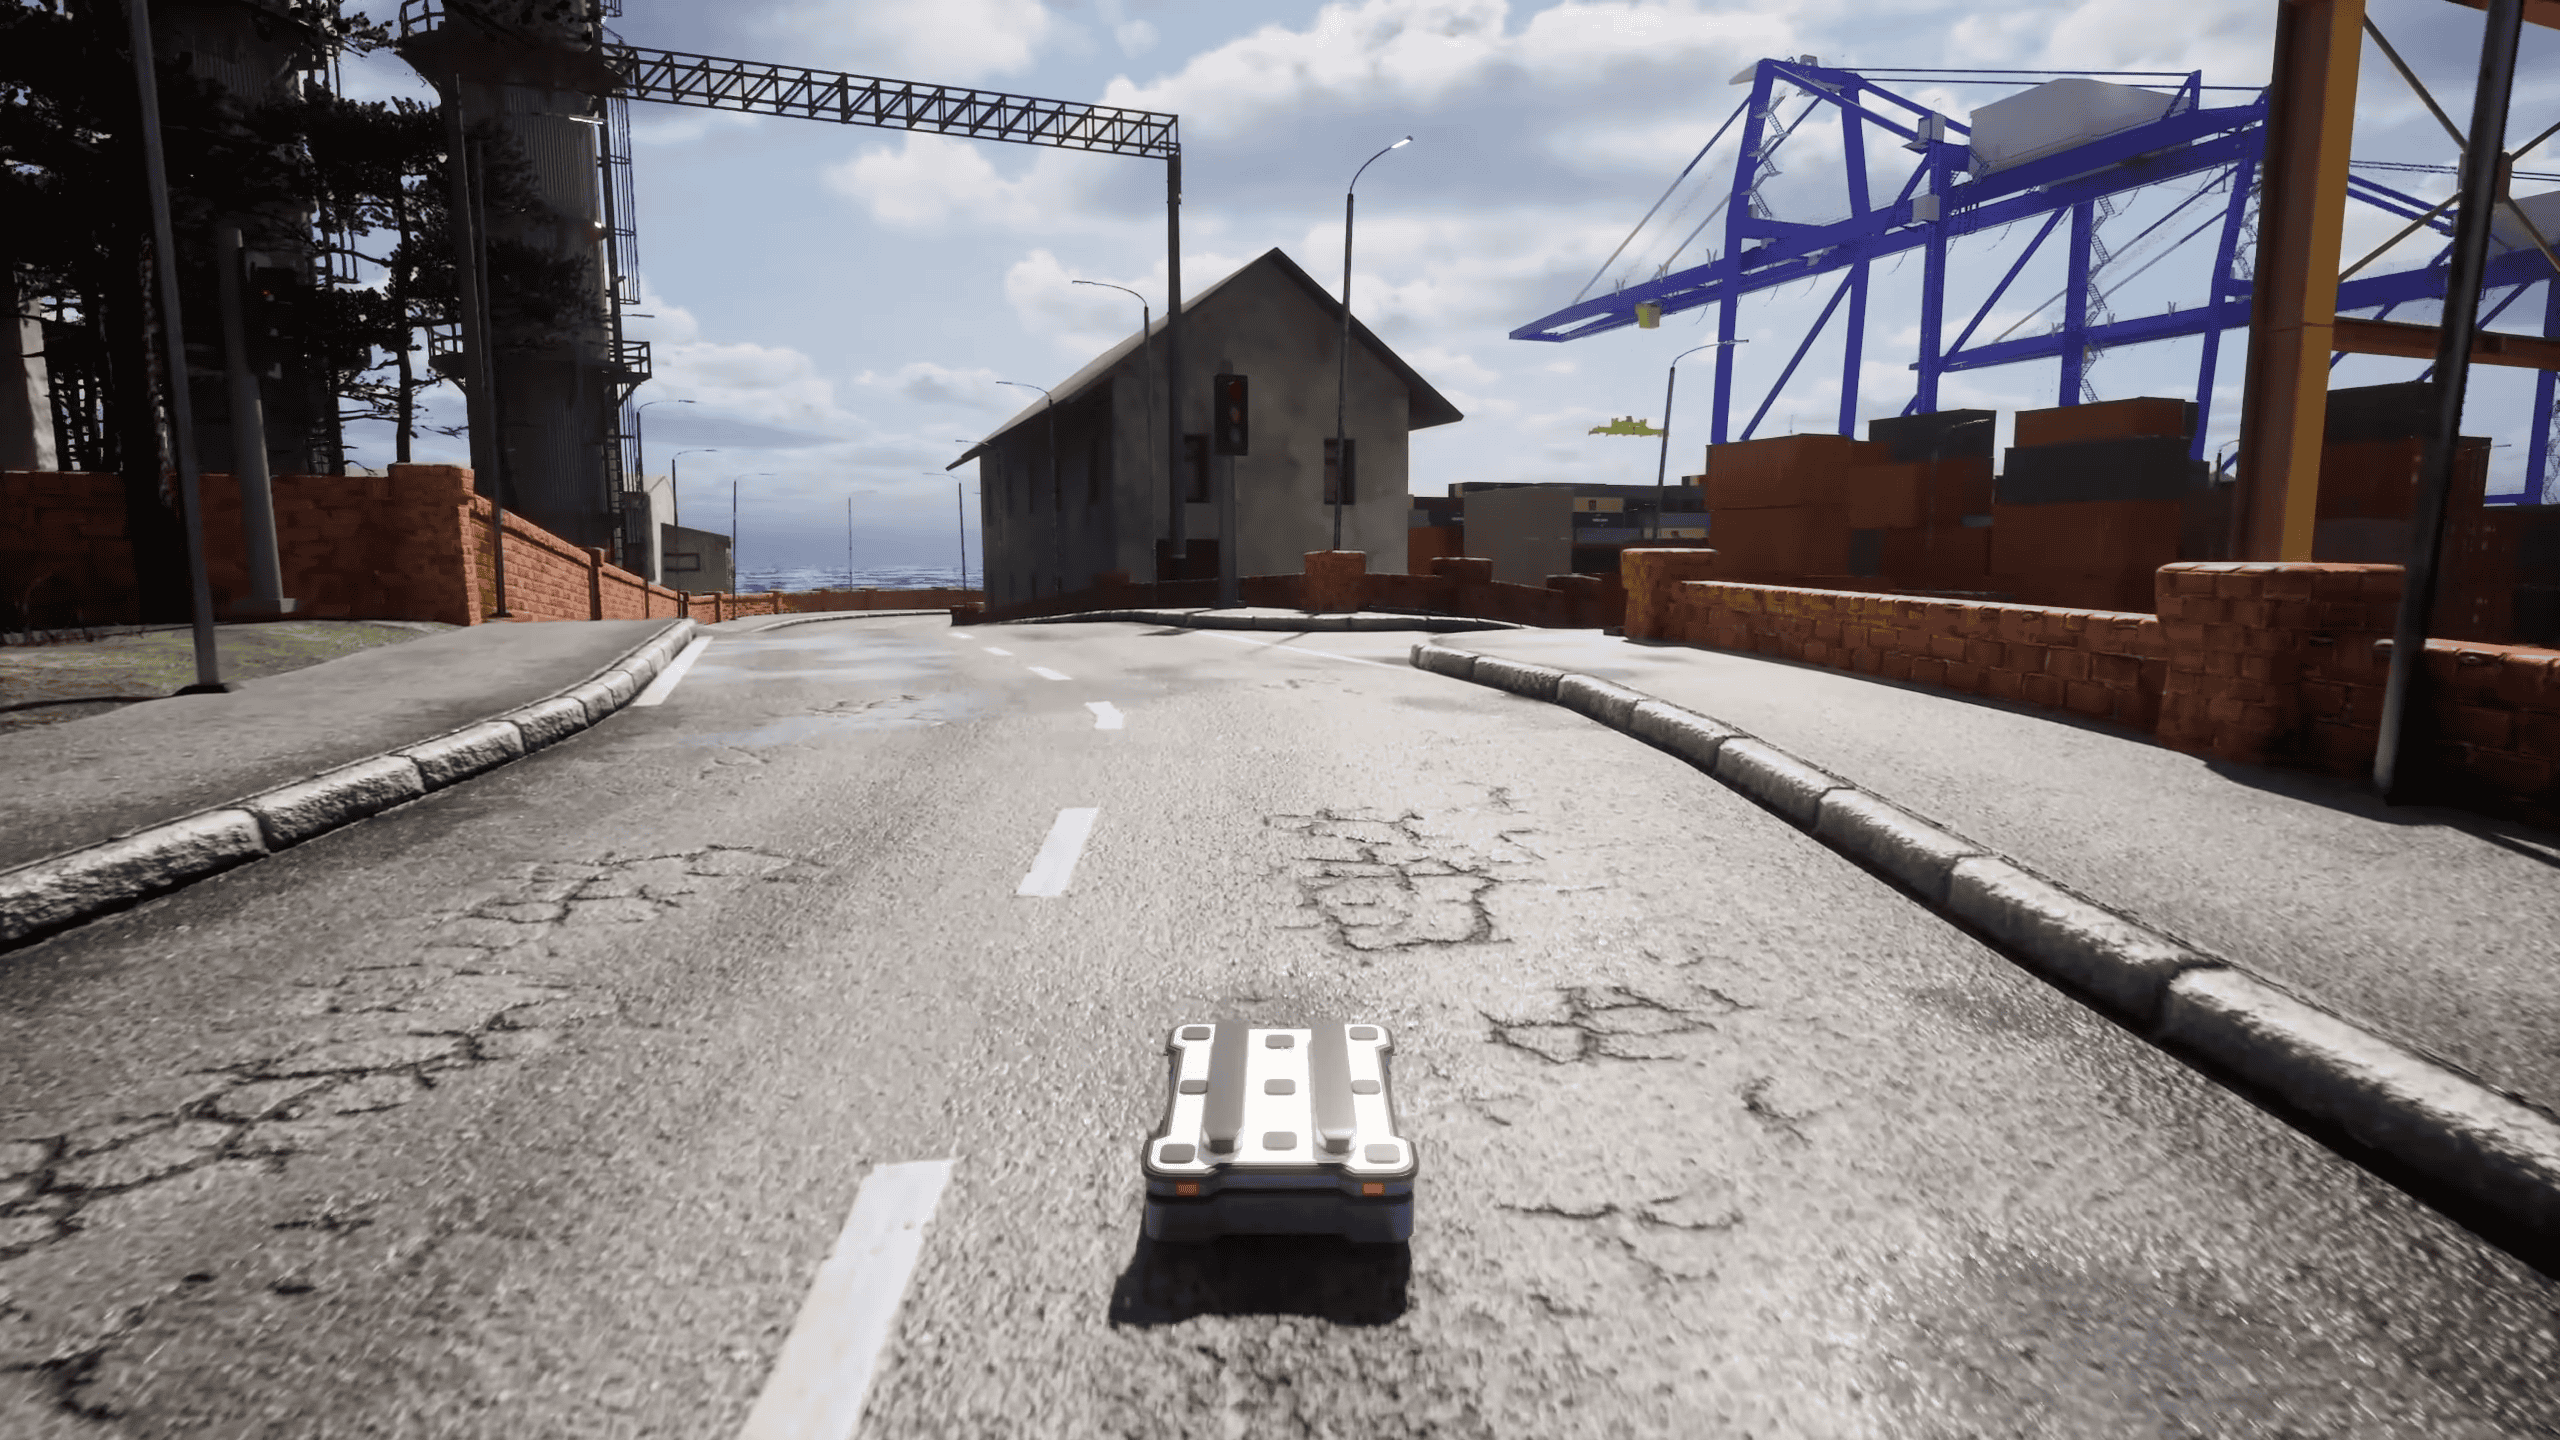
\includegraphics[width=0.4\textwidth]{graphics/Cosys_Airsim_UGV_example.png}
\caption{Example view of a UGV produced by Cosys-AirSim.}
\label{fig:UGV_example_view}
\end{figure}
\noindent
By modifying the underlying architecture to support simulations involving different vehicle domains simultaneously, this project seeks to bridge the gap between simulation and real-world cross-domain deployment. Furthermore, as an extension of an open-source tool, this work contributes to the broader robotics community by providing a flexible, accessible platform for testing cooperative strategies, ultimately reducing the risks and costs associated with physical multi-robot experimentation.
